%% TARGET: Journal of Computing in Civil Engineering (ASCE). ASCE-class draft -- 2026-06-03.
%% Built with the community `ascelike' class (CTAN). For the official ASCE submission,
%% swap \documentclass to the official ascelike-new.cls (same frontmatter structure)
%% and use [Proof]/[NewProof] for the double-spaced review manuscript.
%% Framing: TWO contributions -- (1) a bound-preserving high-resolution compact scheme
%% applied to coastal/ocean tracer transport (METHOD from Li, Xie & Zhang 2018; our
%% contribution = the application + comparison vs the 3rd-order upwind of
%% Sankaranarayanan et al. 1998 + a calibrated mixed-tide SF Bay model); and
%% (2) the expert-guided LLM (Claude Opus 4.8) scientific-computing workflow.
%% KEEP THE SCIENCE HONEST: no method-novelty claim, no oil-spill hindcast claim.
\documentclass[Journal]{ascelike}   %% use [Proof] for the double-spaced review manuscript
\usepackage{amsmath,amssymb,graphicx,booktabs}
\usepackage{algorithm,algpseudocode}
\usepackage{xcolor}
\usepackage{tikz}
\usetikzlibrary{shapes.geometric,arrows.meta,positioning}
\usepackage[round,authoryear]{natbib}
\NameTag{Sankaranarayanan}

\begin{document}
\title{Bound-preserving compact tracer transport in coastal and ocean models:
a case study in expert-guided large-language-model (Claude Opus~4.8)
scientific computing}

\author{S.~Sankaranarayanan\thanks{Independent researcher, thetarho.ai
(corresponding author). Email: sankara68@gmail.com}}
\maketitle

\begin{abstract}
Scalar (salinity, temperature, pollutant) transport in coastal and ocean models is
limited by the discretization of the advective term: high-order schemes produce
unphysical negative concentrations near sharp fronts, while low-order upwind schemes
are excessively diffusive. We apply a bound-preserving high-resolution compact
(Pad\'e) finite-difference scheme---established in the numerical-analysis
literature---to coastal/ocean tracer transport, combining a stable no-flux closure
with an a-posteriori discrete-maximum-principle limiter that keeps the solution within
physical bounds while retaining the compact scheme's resolution. Verified on the
LeVeque deformational-flow benchmark and demonstrated on a calibrated mixed-tide San
Francisco Bay model (six constituents tuned to observed Golden Gate harmonics), it
removes both the negative concentrations of the third-order upwind scheme of a 1998
operational model and the smearing of low-order schemes. As a second, methodological
contribution, the complete study---codes, calibration, experiments, figures, and
manuscript---was developed through an expert-guided, prompt-driven large-language-model
workflow under the author's direction and verification and released as a reproducible
artifact, illustrating that domain expertise, not the model alone, governs scientific
validity.
\end{abstract}

\KeyWords{tracer transport; advection--diffusion; bound-preserving schemes; compact
finite difference; coastal and ocean modeling; deformational flow; mixed tide;
large-language-model workflow.}

%==============================================================
\section{Introduction}
\label{sec:intro}

The transport of salinity, temperature, suspended sediment and dissolved or
particulate pollutants in coastal and ocean waters is governed by the
advection--diffusion equation, and the fidelity of any coastal water-quality,
sediment, oil-spill or biogeochemical model is ultimately limited by how its
advective term is discretized. Two failure modes dominate. Centred (and, more
generally, linear high-order) approximations of the convective term are
non-monotone: near sharp concentration fronts they generate spurious oscillations
and \emph{negative concentrations}, which are not merely cosmetic---negative
tracer values are physically meaningless and can destabilize coupled
biogeochemical or density computations \citep{sankaranarayanan1998}. Low-order
upwind (donor-cell) schemes are, by contrast, unconditionally bounded but
introduce so much numerical diffusion that sharp fronts and filaments are smeared
away within a few grid cells.

The standard compromise in operational coastal models has been to use a
moderately high-order upwind-biased scheme. In the three-dimensional
conservative-pollutant transport model of \citet{sankaranarayanan1998}, a
third-order upwind scheme \citep{kowalik1993} was adopted for the convective
terms specifically to minimize the numerical diffusion of the donor-cell method
while suppressing the negative concentrations produced by central differencing.
Third-order upwinding is a substantial improvement, but it is neither
bound-preserving (it can still overshoot at discontinuities) nor as accurate, for
a given stencil, as the compact (Pad\'e) finite-difference schemes that provide
spectral-like resolution \citep{lele1992}.

In the computational-physics literature these two requirements---high resolution
and guaranteed boundedness---have been reconciled. Maximum-principle-satisfying and
positivity-preserving limiters were developed for finite-volume and discontinuous
Galerkin methods \citep{zhangshu2010,zhangshu2011}, and flux-corrected transport
\citep{zalesak1979} and a-posteriori order-detection (MOOD) \citep{clain2011mood}
provide closely related machinery. More recently, \citet{lixiezhang2018} showed
that the classical compact finite-difference scheme, advanced with strong
stability-preserving time integration, satisfies a weak monotonicity property, so
that a simple limiter enforces strict bounds without sacrificing conservation or
high-order accuracy. These developments have, however, been presented and tested
almost exclusively in the context of compressible gas dynamics and abstract scalar
benchmarks; their relevance to operational coastal and ocean tracer transport,
where the negative-concentration problem was first a practical concern, has not
been demonstrated.

The purpose of this paper is to bring the bound-preserving compact approach to
coastal/ocean tracer transport, as a direct follow-up to
\citet{sankaranarayanan1998}. We (i) present a bound-preserving high-resolution
compact scheme for the advective transport of a tracer---a stable no-flux compact
boundary closure combined with an a-posteriori discrete-maximum-principle
limiter; (ii) quantify its resolution via the modified-wavenumber analysis of
\citet{lele1992}; (iii) verify it on the LeVeque deformational-flow benchmark
\citep{leveque1996}, a stringent test in which a sharp tracer is wound into a thin
filament; and (iv) apply it to tracer transport in a representative tidal-current
field, comparing it against the first- and third-order upwind schemes used in
operational models. The central result is that the bound-preserving compact scheme
removes both pathologies at once: it eliminates the spurious over/undershoots of
the high-order schemes (including the negative concentrations that motivated
\citet{sankaranarayanan1998}) and avoids the excessive smearing of the upwind
schemes, while conserving mass.

The second thread of the paper concerns \emph{how} this model was built. Large
language models (LLMs) such as Claude \citep{anthropic2026claude} have rapidly become
capable of generating scientific and numerical code, and are increasingly used across
computational civil and environmental engineering. They are, however, prone to
producing code that is syntactically correct yet physically wrong: they lack the
domain intuition required to select, for instance, the appropriate tidal forcing,
boundary closures, bottom-friction parameterization, or wetting/drying and stability
safeguards for a coastal hydrodynamic model. This gap---fluent code generation
without physical judgement---is precisely what makes an \emph{expert-in-the-loop} mode
of use necessary, in which a domain expert directs the model and verifies every step
against observations and physics.

A second, methodological contribution is therefore the workflow itself. The complete study---the
compact transport solver, a mixed-tide San Francisco Bay hydrodynamic model
calibrated against observed harmonics, all numerical experiments, and this
manuscript---was produced through an interactive, prompt-driven collaboration with a
large language model (LLM, Claude Opus~4.8) steered by the author's
hydrodynamic-modelling expertise. We argue, and illustrate concretely in
Section~\ref{sec:workflow}, that such expert-in-the-loop LLM workflows are becoming a
practical mode of computational ocean-engineering research---provided domain
knowledge governs the scientific decisions---and we document the process,
including the corrections the expert had to impose, so that it can be assessed and
reused.

The remainder of the paper is organized as follows. Section~\ref{sec:gov}
states the governing equations and the deformational test flow.
Section~\ref{sec:scheme} describes the compact discretization, the stable
boundary closure, and the bound-preserving limiter. Section~\ref{sec:analysis}
presents the modified-wavenumber resolution analysis. Section~\ref{sec:results}
reports the convergence study, the deformational-flow benchmark, and the
mixed-tide San Francisco Bay transport application. Section~\ref{sec:workflow}
documents the expert-guided LLM workflow as a methodological contribution, and
Section~\ref{sec:conclusions} concludes.

%==============================================================
\section{Governing equations and test flow}
\label{sec:gov}

The transport of a passive tracer of concentration $c(x,y,t)$ by a prescribed
velocity field $(u,v)$ is governed by the advection--diffusion equation
\begin{equation}
\frac{\partial c}{\partial t} + u\,\frac{\partial c}{\partial x}
+ v\,\frac{\partial c}{\partial y}
= D\!\left(\frac{\partial^2 c}{\partial x^2}+\frac{\partial^2 c}{\partial y^2}\right),
\label{eq:adv-diff}
\end{equation}
where $D$ is a (constant, isotropic) diffusivity. In coastal and ocean transport
the P\'eclet number is large and the advective term dominates; the discretization
of that term is what produces, or avoids, the unphysical negative concentrations
discussed in Section~\ref{sec:intro}. We therefore focus on the advective limit
($D\to 0$) for the most demanding tests, retaining $D$ where physical diffusion is
relevant.

As a stringent, divergence-free test flow we use the deformational (swirling) flow
of \citet{leveque1996}, defined on the closed unit basin
$\Omega=[0,1]\times[0,1]$ by the streamfunction
\begin{equation}
\psi(x,y,t)=\frac{1}{\pi}\sin^2(\pi x)\,\sin^2(\pi y)\,\cos\!\left(\frac{\pi t}{T}\right),
\label{eq:streamfn}
\end{equation}
giving the non-divergent velocity field
\begin{equation}
u=\frac{\partial\psi}{\partial y}=\sin^2(\pi x)\,\sin(2\pi y)\cos\!\left(\tfrac{\pi t}{T}\right),
\qquad
v=-\frac{\partial\psi}{\partial x}=-\sin(2\pi x)\,\sin^2(\pi y)\cos\!\left(\tfrac{\pi t}{T}\right).
\label{eq:velocity}
\end{equation}
The velocity vanishes on $\partial\Omega$, so the basin is closed; the physically
appropriate boundary condition for a conserved tracer is zero normal flux,
$\partial c/\partial n=0$ on $\partial\Omega$. The factor $\cos(\pi t/T)$ reverses
the flow at $t=T/2$: an initial tracer distribution is progressively stretched and
wound into an ever-thinner filament until $t=T/2$, after which the flow unwinds it.
This benchmark is demanding precisely because it forces a sharp feature through a
strong, time-dependent strain that no low-order scheme can follow without either
smearing it or generating oscillations.

We use two initial conditions. For the resolution and convergence studies a smooth
Gaussian is used. For the bound-preserving tests we use the Zalesak slotted
cylinder---a disk of unit value of radius $R$ centred at $(x_c,y_c)$ with a
rectangular slot of zero value---whose discontinuous edges are the classical probe
for spurious over/undershoots \citep{zalesak1979}.

\section{Bound-preserving compact scheme}
\label{sec:scheme}

\subsection{Compact (Pad\'e) approximation of the first derivative}
\label{sec:compact1}
Compact (Pad\'e) schemes evaluate a derivative implicitly: the nodal derivatives
are coupled through a narrow banded system, which delivers, for a given stencil
width, markedly higher resolution than an explicit difference of the same formal
order \citep{lele1992}. On a uniform mesh $x_i=i h$ with nodal values
$f_i=f(x_i)$, the general tridiagonal family for the first derivative is
\begin{equation}
\alpha f'_{i-1}+f'_{i}+\alpha f'_{i+1}
=a\,\frac{f_{i+1}-f_{i-1}}{2h}+b\,\frac{f_{i+2}-f_{i-2}}{4h}.
\label{eq:compactfam}
\end{equation}
Matching the Taylor expansions of both sides supplies the consistency condition
$a+b=1+2\alpha$ and the fourth-order condition $a+4b=6\alpha$, whose one-parameter
solution is $a=\tfrac23(\alpha+2)$, $b=\tfrac13(4\alpha-1)$; requiring sixth order
adds $a+16b=10\alpha$. The tridiagonal member ($b=0$) therefore fixes
$\alpha=\tfrac14$, $a=\tfrac32$, giving
\begin{equation}
\tfrac14\,f'_{i-1}+f'_{i}+\tfrac14\,f'_{i+1}
=\frac{3}{2}\,\frac{f_{i+1}-f_{i-1}}{2h},
\qquad \alpha=\tfrac14,\ a=\tfrac32,\ b=0,
\label{eq:compact}
\end{equation}
with leading truncation error $\tfrac{1}{120}h^{4}f^{(5)}_i$ (Section~\ref{sec:analysis}).
Setting instead $\alpha=\tfrac13,\,a=\tfrac{14}{9},\,b=\tfrac19$ recovers the
sixth-order tridiagonal member, used here only for the resolution comparison.
Equation~\eqref{eq:compact} forms a tridiagonal system for the vector of nodal
derivatives, solved at $O(N)$ cost per line by the Thomas algorithm and applied
line-by-line in $x$ and $y$ to obtain $\partial c/\partial x$ and
$\partial c/\partial y$.

\subsection{Second derivative for the diffusion term}
\label{sec:compact2}
The diffusion term is discretized with the companion fourth-order compact
second-derivative scheme \citep{lele1992}
\begin{equation}
\tfrac{1}{10}\,f''_{i-1}+f''_{i}+\tfrac{1}{10}\,f''_{i+1}
=\frac{6}{5}\,\frac{f_{i+1}-2f_i+f_{i-1}}{h^{2}},
\label{eq:compact2}
\end{equation}
whose leading error is $-\tfrac{1}{20}h^{4}f^{(6)}_i$ and which shares the
spectral-like resolution of \eqref{eq:compact} (Fig.~\ref{fig:wavenumber2}). In
the advection-dominated tests below ($D\to0$) this term is inactive; it is retained
for completeness and for problems where physical diffusion matters.

\subsection{A stable no-flux boundary closure}
\label{sec:bc}
At a closed (no-flow) wall the physical condition $\partial c/\partial n=0$ makes
the normal derivative vanish, so we impose $f'=0$ at the boundary nodes directly
and solve \eqref{eq:compact} for the interior derivatives. This is both physically
consistent and numerically stable, in contrast to the one-sided (extrapolation)
compact closures \citep{lele1992,carpenter1993}, which we found to drive a weak
boundary instability for the present pure-advection problem. The semi-discrete
system is advanced with the classical fourth-order Runge--Kutta method, which (as a
strong-stability-preserving-compatible explicit integrator) is what the
bound-preserving theory of \citet{lixiezhang2018} requires.

\subsection{Upwind schemes used for comparison}
\label{sec:upwind}
We benchmark the compact scheme against the two upwind discretizations that
bracket operational coastal-model practice. With $u^{\pm}=\tfrac12(u\pm|u|)$, the
first-order upwind (donor-cell) approximation of the advective term is
\begin{equation}
u_i\Big(\frac{\partial c}{\partial x}\Big)_i \approx
u_i^{+}\,\frac{c_i-c_{i-1}}{h}+u_i^{-}\,\frac{c_{i+1}-c_i}{h},
\label{eq:up1}
\end{equation}
which is monotone (hence strictly bounded) but introduces a numerical diffusion of
coefficient $\tfrac12|u|h$ that smears sharp fronts. The third-order upwind-biased
scheme adopted in the transport model of \citet{sankaranarayanan1998}, following
\citet{kowalik1993}, is
\begin{equation}
\Big(\frac{\partial c}{\partial x}\Big)_i \approx \frac{1}{6h}
\begin{cases}
\;2c_{i+1}+3c_i-6c_{i-1}+c_{i-2}, & u_i>0,\\[4pt]
-c_{i+2}+6c_{i+1}-3c_i-2c_{i-1}, & u_i<0,
\end{cases}
\label{eq:up3}
\end{equation}
whose leading error is dispersive ($\sim\!\tfrac{1}{12}h^{3}\partial^4_x c$) rather
than diffusive. It is far sharper than donor-cell, but---being linear and
non-monotone---it does not satisfy a maximum principle and overshoots at
discontinuities, producing the negative concentrations noted by
\citet{sankaranarayanan1998} and quantified in Section~\ref{sec:results}.

\subsection{A-posteriori bound-preserving limiter}
\label{sec:limiter}
A linear high-order scheme such as \eqref{eq:compact} is non-monotone and produces
Gibbs oscillations at discontinuities. To enforce strict bounds we use an
a-posteriori limiting strategy, following the now-standard approach of detecting
constraint violations after a candidate update and blending toward a monotone
low-order update \citep{zalesak1979,clain2011mood,lixiezhang2018}. Let $c^{HO}$ be
the compact Runge--Kutta update at a node, and let $c^{LO}$ be the first-order
upwind update \eqref{eq:up1} over the same step, which is bounded by the local data
under the usual CFL restriction. Denoting by $[\,c_{\min},c_{\max}\,]$ the discrete
local maximum-principle bounds (the minimum and maximum of $c$ over the node's
neighbourhood $\mathcal{N}(i)$ at the previous step), the limited update is
\begin{equation}
c = c^{LO} + \theta\,(c^{HO}-c^{LO}),
\qquad
\theta=\min\!\Big(1,\ \tfrac{c_{\max}-c^{LO}}{c^{HO}-c^{LO}}\Big)\ \text{or}\
\min\!\Big(1,\ \tfrac{c^{LO}-c_{\min}}{c^{LO}-c^{HO}}\Big),
\label{eq:limiter}
\end{equation}
according to the sign of $c^{HO}-c^{LO}$, with $\theta\in[0,1]$. By construction
$c\in[c_{\min},c_{\max}]$, so the discrete solution never leaves the physical
bounds, while in smooth regions $\theta\to1$ and the spectral-like compact
resolution is retained. The complete time step is summarized in
Algorithm~\ref{alg:bp}. We emphasise that this limiting strategy is taken from the
literature \citep{lixiezhang2018}; the contribution of the present paper is its
application to, and assessment for, coastal/ocean tracer transport.

\begin{algorithm}[t]
\caption{One bound-preserving compact time step $c^{n}\!\to c^{n+1}$.}
\label{alg:bp}
\begin{algorithmic}[1]
\Require nodal field $c^{n}$ with $c^{n}_i\in[0,1]$
\State $c^{HO}\gets$ compact (Pad\'e) RK4 advance of \eqref{eq:adv-diff} using
       \eqref{eq:compact}, \eqref{eq:compact2} and the closure of \S\ref{sec:bc}
\State $c^{LO}\gets$ first-order upwind \eqref{eq:up1} advance over the same $\Delta t$
\For{each node $i$}
  \State $c_{\min}\gets\min_{j\in\mathcal{N}(i)}c^{n}_j$,\quad
         $c_{\max}\gets\max_{j\in\mathcal{N}(i)}c^{n}_j$
  \If{$c^{HO}_i>c_{\max}$ \textbf{or} $c^{HO}_i<c_{\min}$}
     \State pick $\theta_i\in[0,1]$ from \eqref{eq:limiter} so that $c^{n+1}_i\in[c_{\min},c_{\max}]$
  \Else
     \State $\theta_i\gets1$ \Comment{accept the high-order update}
  \EndIf
  \State $c^{n+1}_i\gets c^{LO}_i+\theta_i\,(c^{HO}_i-c^{LO}_i)$
\EndFor
\Ensure $c^{n+1}_i\in[c_{\min},c_{\max}]\subseteq[0,1]$
\end{algorithmic}
\end{algorithm}

\section{Resolution analysis}
\label{sec:analysis}

The advantage of the compact scheme over a conventional finite difference of the
same order is best seen through the modified-wavenumber (Fourier) analysis of
\citet{lele1992}. Substituting a Fourier mode $f_j=\exp(\mathrm{i}\,k\,j h)$ into
\eqref{eq:compact} gives the modified wavenumber
\begin{equation}
k'h=\frac{a\,\sin(kh)}{1+2\alpha\cos(kh)}
   =\frac{\tfrac32\sin(kh)}{1+\tfrac12\cos(kh)},
\label{eq:modwave}
\end{equation}
which a symbolic (computer-algebra) expansion confirms matches the exact
wavenumber to fourth order, $k'h-kh=-\tfrac{1}{180}(kh)^5+\mathcal{O}((kh)^7)$,
consistent with the leading truncation error $\tfrac{1}{120}h^4 f^{(5)}$ of
\eqref{eq:compact} \citep{lele1992}. Figure~\ref{fig:wavenumber} compares the
modified wavenumber and the dispersion error of the compact scheme with
second-, fourth- and sixth-order central differences. The compact scheme follows
the exact differentiation over a substantially wider band of wavenumbers: its
resolving efficiency (the largest $kh$ for which $|k'h-kh|/\pi<0.01$) is
$0.43\pi$, against $0.32\pi$ for the standard fourth-order central scheme. This
``spectral-like'' resolution is what allows the scheme to carry the thin filaments
of the deformational flow with little numerical dispersion.

\begin{figure}[t]\centering
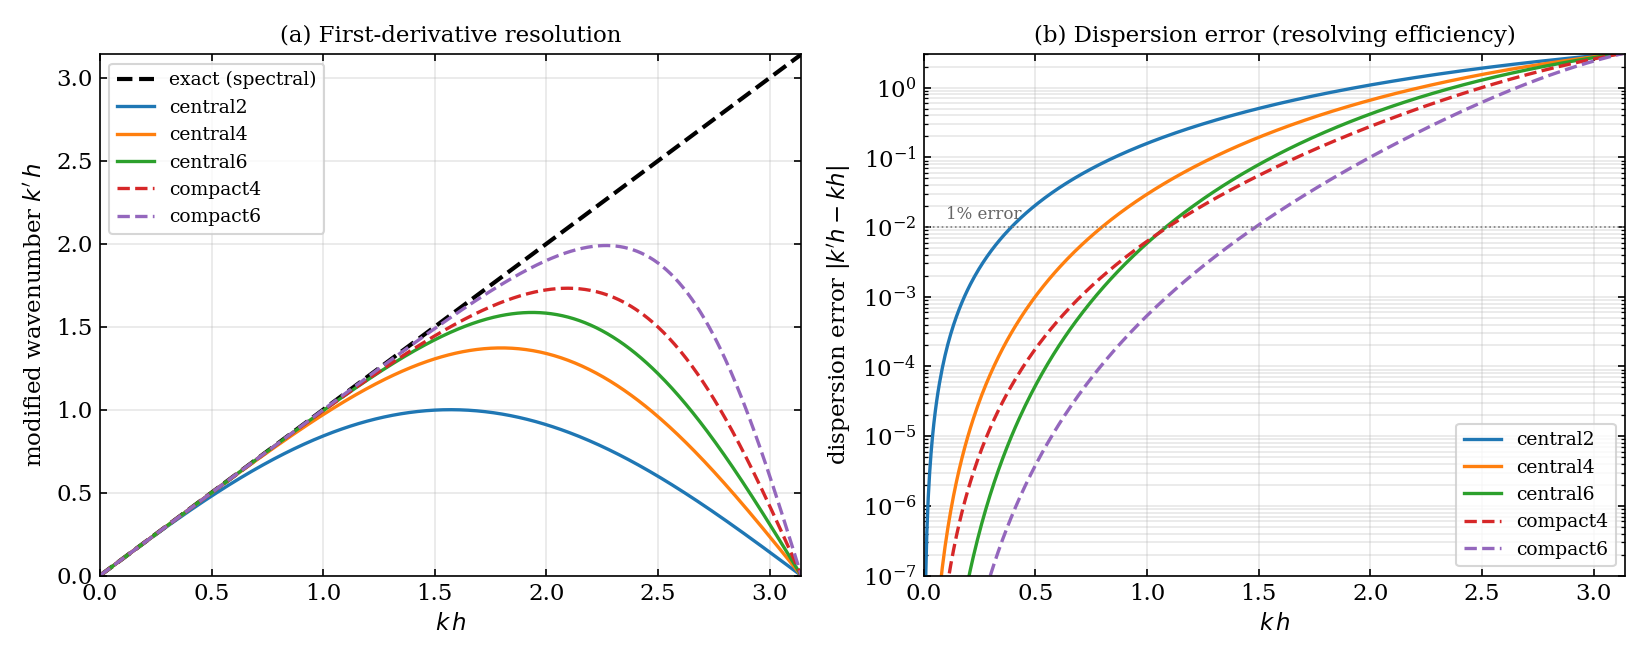
\includegraphics[width=\linewidth]{figures/fig1_wavenumber_analysis.png}
\caption{Resolution of the first-derivative approximations. (a) Modified
wavenumber $k'h$ versus $kh$; (b) dispersion error $|k'h-kh|$ (log scale). The
compact scheme stays close to exact differentiation (dashed) over a wider band
than central schemes of equal or higher order. After \citet{lele1992}.}
\label{fig:wavenumber}
\end{figure}

The companion compact second-derivative scheme \eqref{eq:compact2} has the modified
wavenumber $\widetilde{k^2}h^2=\tfrac{12}{5}(1-\cos kh)/(1+\tfrac15\cos kh)$, which
likewise tracks the exact $(kh)^2$ to fourth order and over a much wider band than
the standard three-point second difference (Fig.~\ref{fig:wavenumber2}). The
diffusion operator therefore inherits the same spectral-like fidelity as the
advection operator.

\begin{figure}[t]\centering
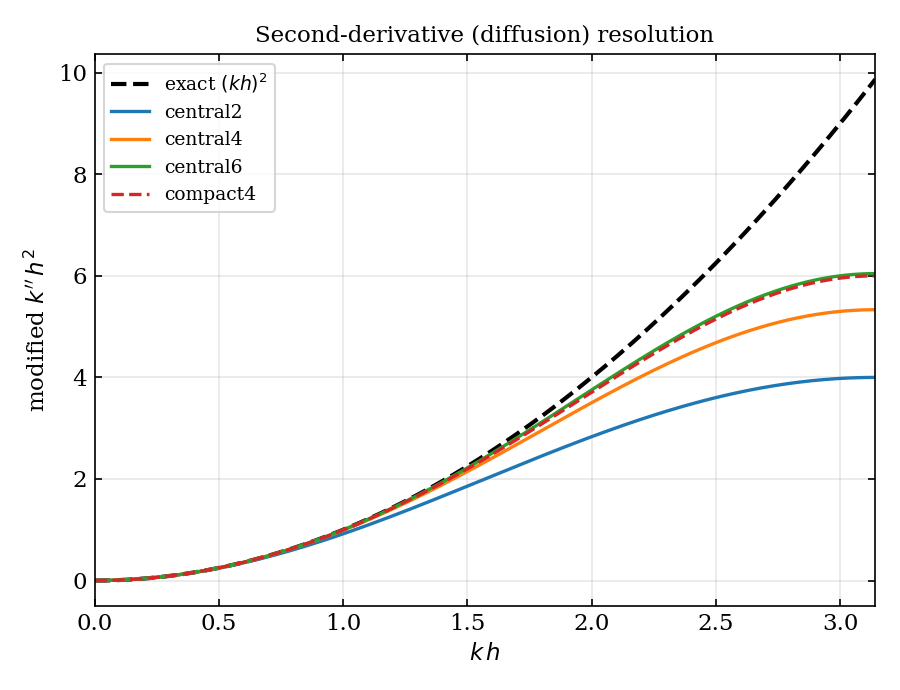
\includegraphics[width=\linewidth]{figures/fig2_second_derivative_wavenumber.png}
\caption{Resolution of the second-derivative approximations: modified wavenumber
$\widetilde{k^2}h^2$ and its error for the fourth-order compact scheme
\eqref{eq:compact2} versus standard central second differences. After
\citet{lele1992}.}
\label{fig:wavenumber2}
\end{figure}

\section{Results}
\label{sec:results}

\subsection{Convergence}
\label{sec:conv}
The formal accuracy of the compact discretization and its no-flux closure is
confirmed by differentiating a Neumann-compatible test function on successively
refined grids. The compact scheme \eqref{eq:compact} attains its design
fourth-order rate (measured slope $4.00$ over $N=33$ to $513$), as do the
second- and sixth-order central schemes used for comparison
(Fig.~\ref{fig:convergence}). The stable Neumann closure does not degrade the
interior order, and the time integration with RK4 reproduces a pure-advection
deformation-and-reversal cycle to a relative error of order $10^{-9}$, confirming
that the advection operator and boundary treatment are correct.

\begin{figure}[t]\centering
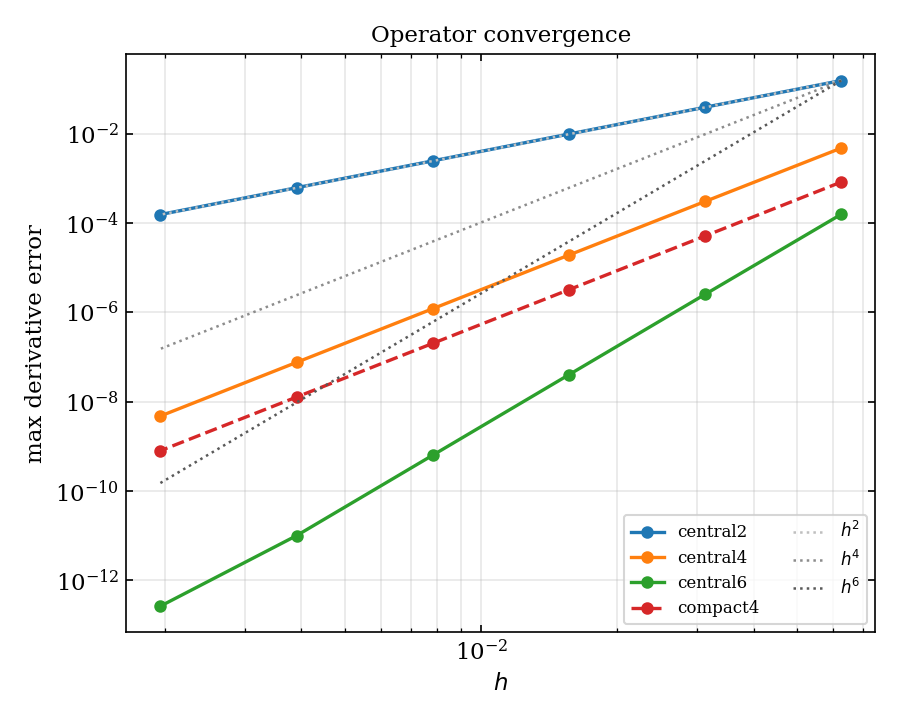
\includegraphics[width=0.62\linewidth]{figures/fig3_convergence.png}
\caption{Operator convergence: maximum derivative error versus grid spacing for
second-, fourth- and sixth-order central schemes and the fourth-order compact
scheme, with reference slopes.}
\label{fig:convergence}
\end{figure}

\subsection{Deformational-flow benchmark}
\label{sec:deform}
The bound-preserving property is assessed on the LeVeque deformational flow with a
slotted-cylinder initial condition, in the advection-dominated regime where the
discontinuous edges are most demanding. Figure~\ref{fig:slotted} shows the field at
maximum deformation. First-order upwind is bounded but has diffused the feature
beyond recognition; third-order upwind is sharper but overshoots
($[-0.08,1.11]$); the plain compact scheme rings with large Gibbs oscillations
($[-0.56,1.45]$); only the bound-preserving compact scheme is simultaneously sharp
and strictly bounded in $[0,1]$. A cross-section through the filament
(Fig.~\ref{fig:cross}) makes the over- and undershoots explicit. Quantitatively
(Table~\ref{tab:deform}), the bound-preserving compact scheme attains the smallest
relative $L_2$ error of any bounded scheme and retains most of the high-concentration
overlap of the unlimited compact scheme (IoU $0.88$ vs.\ $0.93$)---far exceeding the
diffusive first-order upwind result (IoU $0.65$)---while being the only
high-resolution scheme that never leaves the physical bounds. Its slightly lower IoU
than the unlimited compact scheme is the modest, expected price of strict boundedness.

\begin{figure}[t]\centering
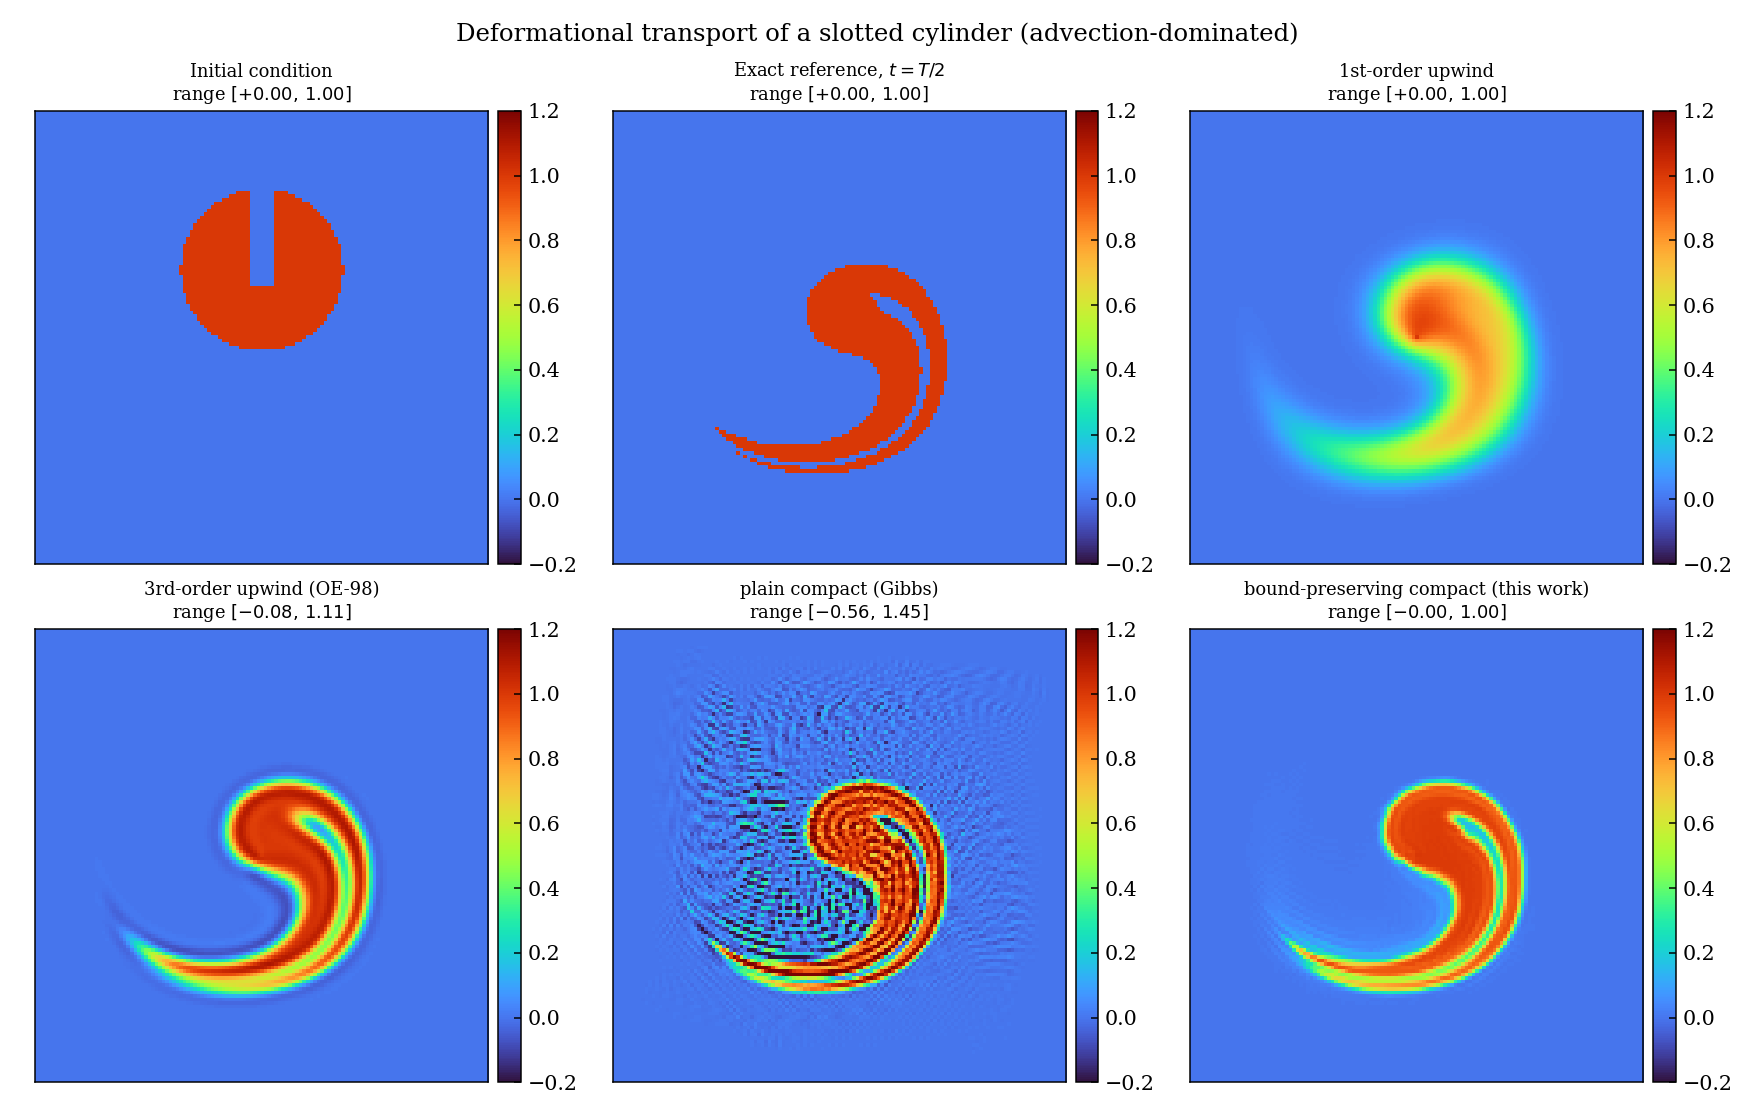
\includegraphics[width=\linewidth]{figures/fig4_slotted_cylinder_panels.png}
\caption{Deformational transport of a slotted cylinder at maximum deformation.
Plain high-order schemes overshoot/undershoot; first-order upwind smears; the
bound-preserving compact scheme is sharp and bounded.}
\label{fig:slotted}
\end{figure}

\begin{figure}[t]\centering
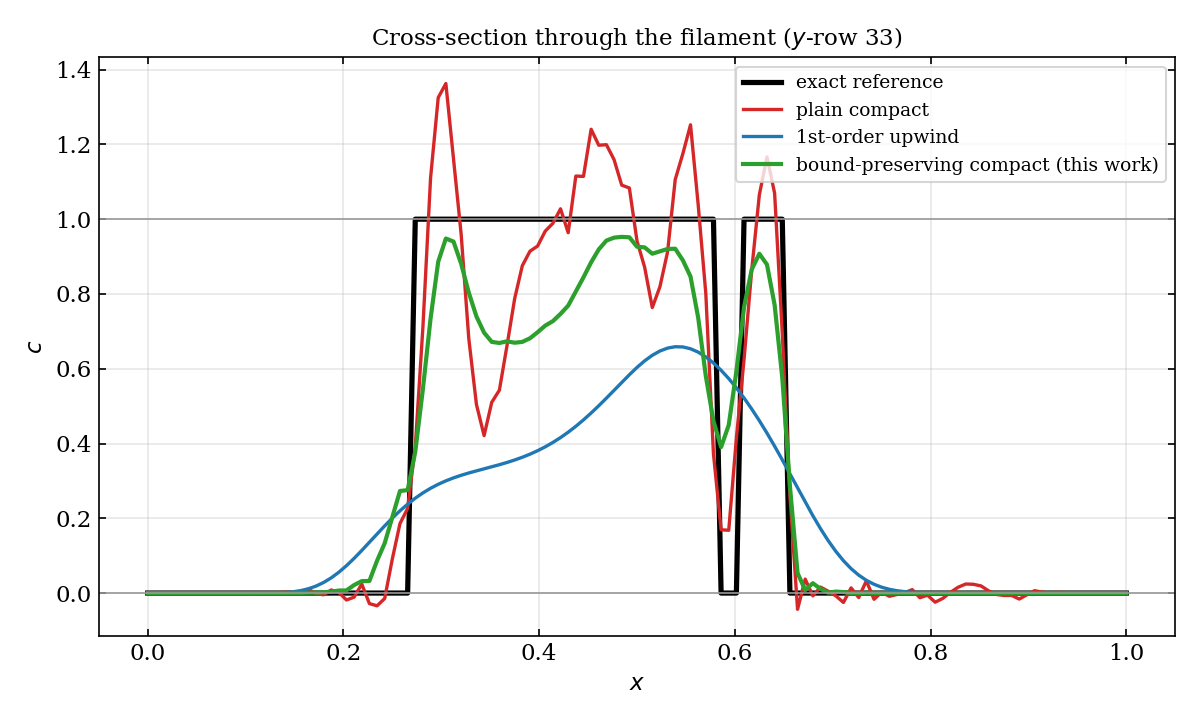
\includegraphics[width=0.7\linewidth]{figures/fig5_cross_section.png}
\caption{Cross-section through the deformed filament. The plain compact scheme
exceeds $[0,1]$; first-order upwind is heavily smeared; the bound-preserving
compact scheme tracks the sharp profile within bounds.}
\label{fig:cross}
\end{figure}

\begin{table}[t]\centering
\caption{Deformational benchmark (slotted cylinder, maximum deformation,
$N=129$): relative $L_2$ error, range, and high-concentration IoU.}
\label{tab:deform}
\begin{tabular}{lccc}
\toprule
scheme & rel.\ $L_2$ & $[\min,\max]$ & IoU($c>0.5$)\\
\midrule
1st-order upwind            & 0.528 & $[\phantom{-}0.00,\,1.00]$ & 0.65\\
3rd-order upwind (1998)      & 0.317 & $[-0.08,\,1.11]$ & 0.92\\
plain compact               & 0.336 & $[-0.56,\,1.45]$ & 0.93\\
\textbf{bound-preserving compact} & \textbf{0.310} & $[\phantom{-}0.00,\,1.00]$ & 0.88\\
\bottomrule
\end{tabular}
\end{table}

\subsection{Application: tracer transport in San Francisco Bay}
\label{sec:sfbay}
To demonstrate the scheme in an operational coastal setting we transport a tracer
in the tidal-current field of San Francisco Bay, the site of the 2007 \emph{Cosco
Busan} oil spill. On 7 November 2007 the container ship \emph{Cosco Busan} struck
the San Francisco--Oakland Bay Bridge in heavy fog, rupturing a fuel tank and
releasing about $53{,}000$ gallons (roughly $200$~t) of heavy IFO-380 bunker fuel
into the bay; wind and tide spread the oil to the Golden Gate, the Marin shorelines
and the outer-coast beaches, oiling more than $3{,}000$ acres (about $200$~miles) of
shoreline and causing documented injury to Pacific herring spawning habitat and
seabirds \citep{noaacoscobusan,incardona2012pnas,incardona2012plos}. The spill
motivates the present test: a sharp patch of tracer is released at the allision
point ($122.357^\circ$W, $37.806^\circ$N) and advected by the depth-averaged tidal
currents over the bay bathymetry (Fig.~\ref{fig:domain}). The bathymetry is taken
from the NOAA Coastal Relief Model ($3$~arc-second, $\sim\!90$~m) regridded to a
uniform $200$~m mesh that resolves the deep ($\sim\!90$~m) Golden Gate strait; the
model domain covers the Central and North (San Pablo) Bay---the region affected by
the spill. The depth-averaged currents are generated by a semi-implicit
($\theta$-method) shallow-water solver of the Casulli type
\citep{casulli1990,casulli1992}, in which the free-surface gravity-wave terms are
treated implicitly---removing the restrictive surface-wave CFL limit---while
advection and bottom friction are treated explicitly. Bottom friction uses a
depth-dependent (Manning) drag $C_d=g\,n^2/H^{1/3}$ with $n=0.037$, giving
$C_d\approx0.003$ in the deep channels (consistent with the calibration of
\citealp{sankaranarayanan2003}) and larger drag over the shoals; a minimum depth of
$3$~m is imposed so that no cell dries over the tidal cycle, which preserves
numerical stability.

San Francisco Bay has a \emph{mixed, predominantly semidiurnal} tide: the diurnal
constituents are comparable to the semidiurnal ones, producing the characteristic
\emph{diurnal inequality} (successive high and low waters of unequal height). The
model is therefore forced at the Pacific open boundary by the six dominant
constituents---the semidiurnal $M_2$, $S_2$, $N_2$ and the diurnal $K_1$, $O_1$,
$P_1$---with amplitudes calibrated, band by band, to the NOAA Golden Gate harmonic
constants (station~9414290) and phases set to the NOAA epochs. The resulting Golden
Gate tide reproduces the observed harmonics (e.g.\ $M_2$ amplitude $0.58$~m vs.\
observed $0.58$~m; $O_1$ $0.22$ vs.\ $0.23$~m) and the mixed character (form factor
$(K_1{+}O_1)/(M_2{+}S_2)\approx0.9$), including the diurnal inequality
(Fig.~\ref{fig:tide}).

We further validate the currents against the observationally-validated tidal model
of the same bay by \citet{sankaranarayanan2003}, whose boundary-fitted
depth-averaged model was verified against NOAA/SFPORTS data ($M_2$ surface
elevation within $8$~cm and $8^\circ$ at $24$ stations; depth-averaged currents
within $11\%$ RMS, correlation $>0.95$). The model reproduces the Golden Gate $M_2$
principal current amplitude of $0.96$~m\,s$^{-1}$ (observed $1.1$~m\,s$^{-1}$, within
the $0.2$~m\,s$^{-1}$ current error reported for the validated model).
Table~\ref{tab:currents} compares the principal $M_2$ current amplitudes (observed
values from the $90$-day harmonic analysis of Cheng et al., reported by
\citealp{sankaranarayanan2003}) at the two stations with published current
harmonics. A single simulation records the depth-averaged current at four stations;
the resulting time series (Fig.~\ref{fig:currents}) show the mixed-tide modulation
(unequal successive maxima---the diurnal inequality in the currents) and the
expected decrease from the Golden Gate into the bay. Full details of the
hydrodynamic calibration are given in the supplementary calibration note. The tracer
transport below is carried by this mixed-tide field.

\begin{figure}[t]\centering
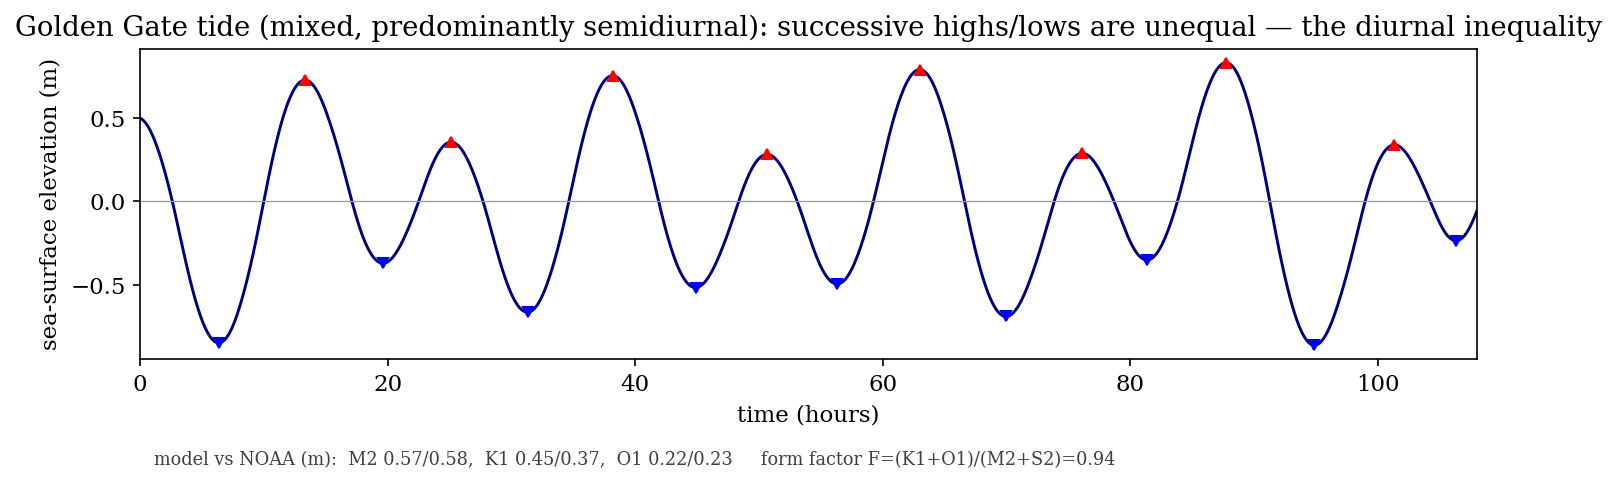
\includegraphics[width=0.9\linewidth]{figures/fig_sfbay_tide.png}
\caption{Modelled Golden Gate sea-surface elevation over $4.5$ days. The tide is
mixed (semidiurnal $+$ diurnal): successive highs (\textcolor{red}{$\triangle$})
and lows (\textcolor{blue}{$\triangledown$}) are unequal---the diurnal
inequality---with constituent amplitudes calibrated to the NOAA Golden Gate
harmonics (station~9414290).}
\label{fig:tide}
\end{figure}

\begin{table}[t]\centering
\caption{Tidal forcing constituents (NOAA Golden Gate station~9414290) and the
modelled Golden Gate surface-elevation amplitude. N$_2$, K$_1$ and P$_1$ are forced
at their observed amplitudes but are not separable from M$_2$/each other in a
$\sim\!16$-day record; the cleanly separable constituents (M$_2$, S$_2$, O$_1$) match
the observations. Bottom friction: Manning $n=0.037$; minimum depth $3$~m.}
\label{tab:tide}
\begin{tabular}{lccc}
\toprule
constituent & band & NOAA amp.\ (m) & model amp.\ (m)\\
\midrule
M$_2$ & semidiurnal & 0.576 & 0.57\\
S$_2$ & semidiurnal & 0.137 & 0.14\\
N$_2$ & semidiurnal & 0.122 & ---\\
K$_1$ & diurnal     & 0.370 & ---\\
O$_1$ & diurnal     & 0.230 & 0.22\\
P$_1$ & diurnal     & 0.114 & ---\\
\bottomrule
\end{tabular}
\end{table}

\begin{table}[t]\centering
\caption{Principal $M_2$ depth-averaged current amplitude: observations
(\citealp{sankaranarayanan2003}, after the harmonic analysis of Cheng et al.,
1993) versus the present calibrated $200$~m model.}
\label{tab:currents}
\begin{tabular}{lcc}
\toprule
station & observed $M_2$ amp.\ (m\,s$^{-1}$) & present model (m\,s$^{-1}$)\\
\midrule
Golden Gate (C1) & 1.1 & 0.96\\
Oakland          & 0.6 & 0.53\\
\bottomrule
\end{tabular}
\end{table}

\begin{figure}[t]\centering
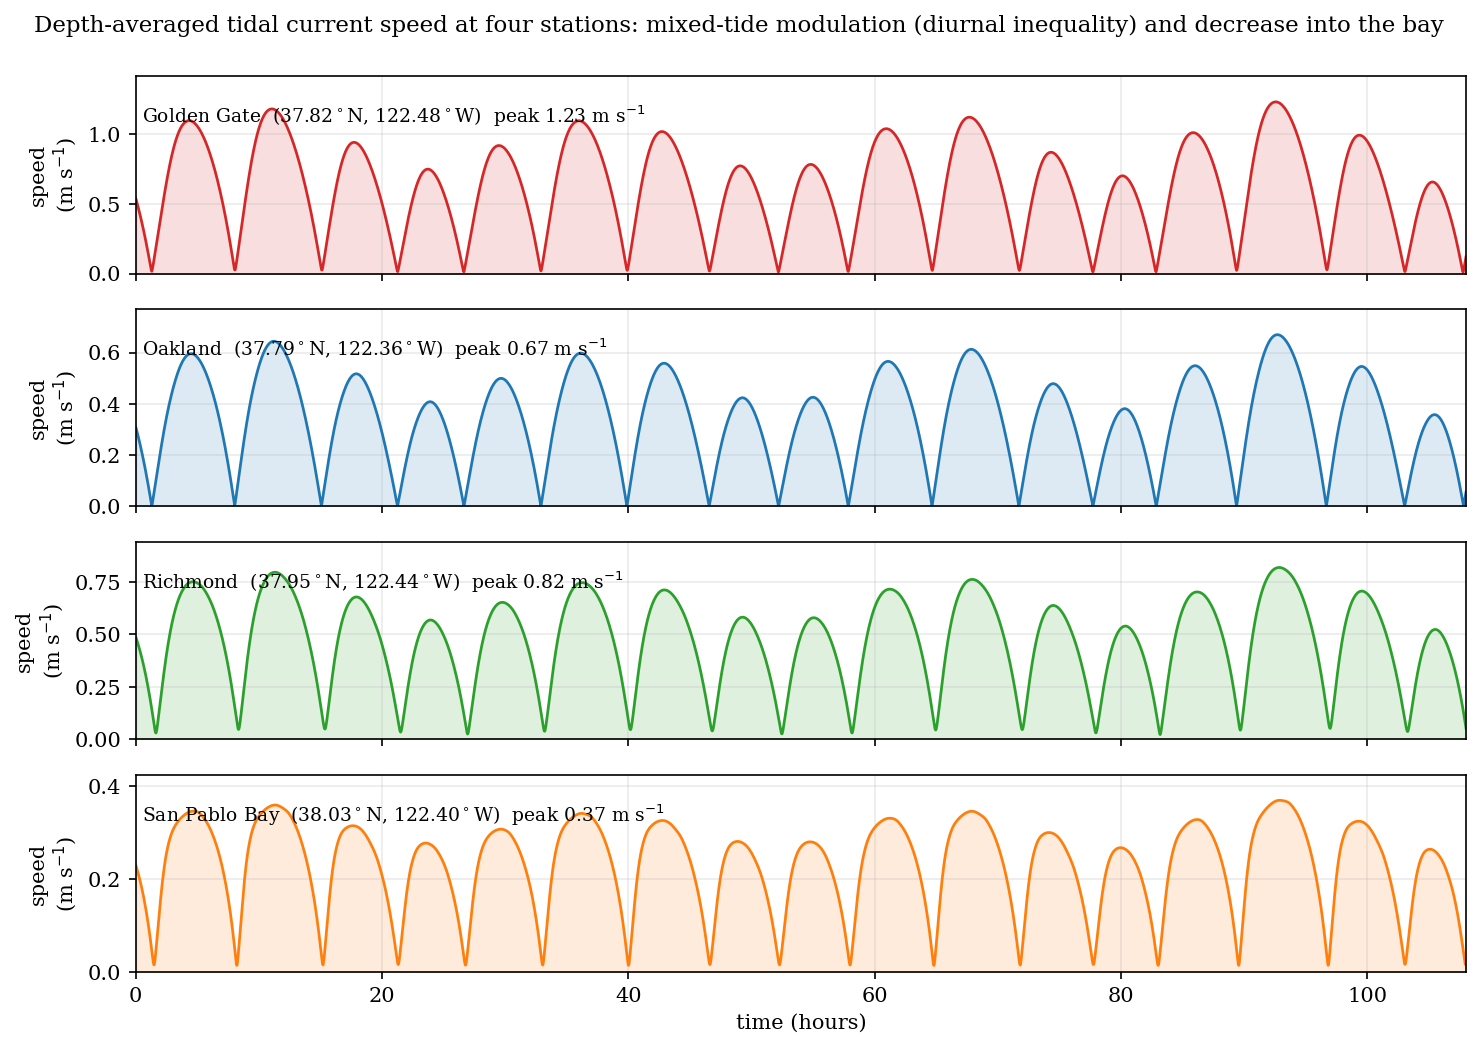
\includegraphics[width=0.92\linewidth]{figures/fig_sfbay_currents.png}
\caption{Depth-averaged tidal current speed at four stations over $4.5$ days, from a
single mixed-tide simulation. Successive flood/ebb maxima are unequal (the diurnal
inequality), and the current decreases from the Golden Gate into the bay. Peak
speeds: Golden Gate $1.2$, Richmond $0.8$, Oakland $0.7$, San Pablo Bay
$0.4$~m\,s$^{-1}$.}
\label{fig:currents}
\end{figure}

Figure~\ref{fig:sfbay} compares the schemes after five hours of tidal transport on
the $200$~m grid. The result mirrors, in a realistic flow, the behaviour identified
in \citet{sankaranarayanan1998}: the third-order upwind scheme adopted there
develops \emph{negative concentrations} ($\min=-0.17$) at the patch edges, and the
plain compact scheme oscillates strongly ($[-2.6,\,3.0]$). First-order upwind
stays bounded but is strongly diffusive, smearing the sharp patch edges. Only the
bound-preserving compact scheme is simultaneously sharp and strictly within
$[0,1]$. Negative tracer concentrations of the magnitude produced by the
third-order upwind scheme are not merely cosmetic in a spill or water-quality
context---they corrupt subsequent weathering, dissolution and density
computations---which is precisely why their elimination, at high resolution, is
valuable.

We emphasise that this is a demonstration of the transport scheme in a realistic,
observationally-calibrated tidal field---\emph{not} a hindcast of the \emph{Cosco
Busan} oil trajectory. The observed oil drift was wind-driven (windage of order
$3\%$ of the wind speed, plus Stokes drift) and involved evaporation, emulsification
and shoreline stranding; reproducing it would additionally require the winds of
$7$--$13$ November $2007$ and a coupled wind-driven trajectory/weathering model such
as those used operationally during the response \citep[e.g.\ the GNOME
model,][]{beeglekrause2001gnome}, which are outside the present scope. The tracer
here is passive and tide-advected, and the comparison isolates the behaviour of the
advection schemes.

\begin{figure}[t]\centering
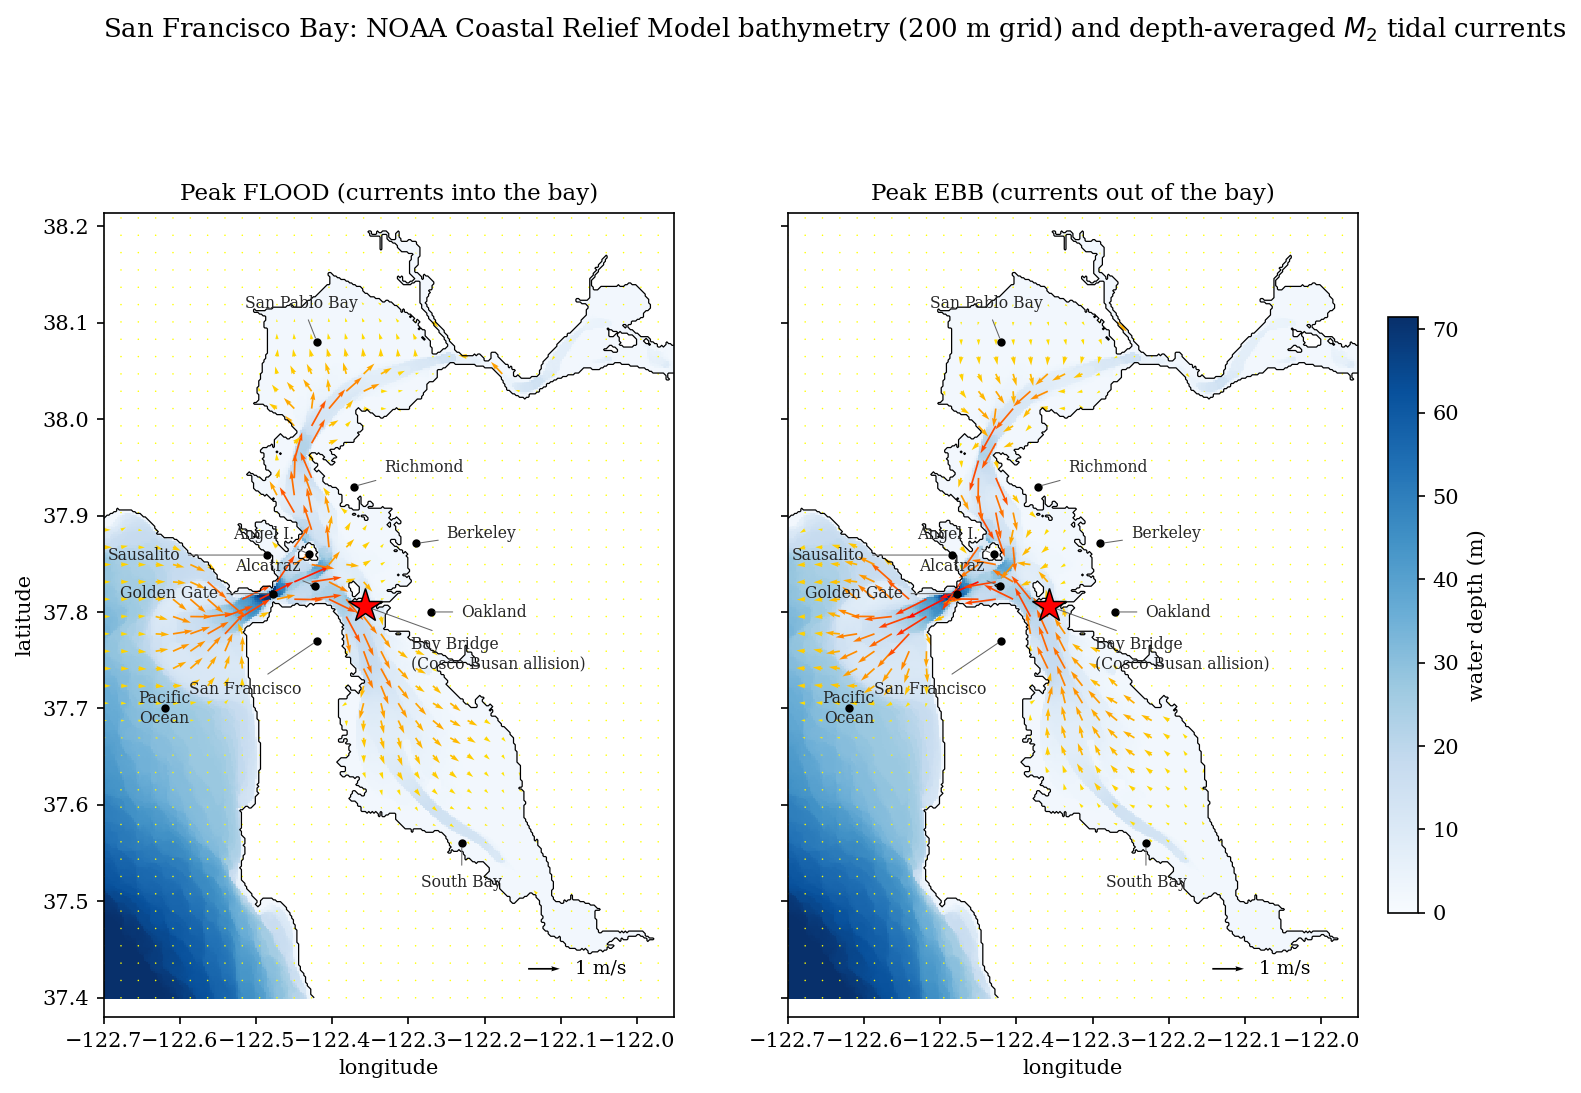
\includegraphics[width=\linewidth]{figures/fig_sfbay_domain.png}
\caption{San Francisco Bay: NOAA Coastal Relief Model bathymetry on the $200$~m
grid, with landmarks and the depth-averaged $M_2$ tidal currents at peak flood
(left) and peak ebb (right). The \emph{Cosco Busan} allision (tracer-release)
point at the Bay Bridge is starred.}
\label{fig:domain}
\end{figure}

\begin{figure}[t]\centering
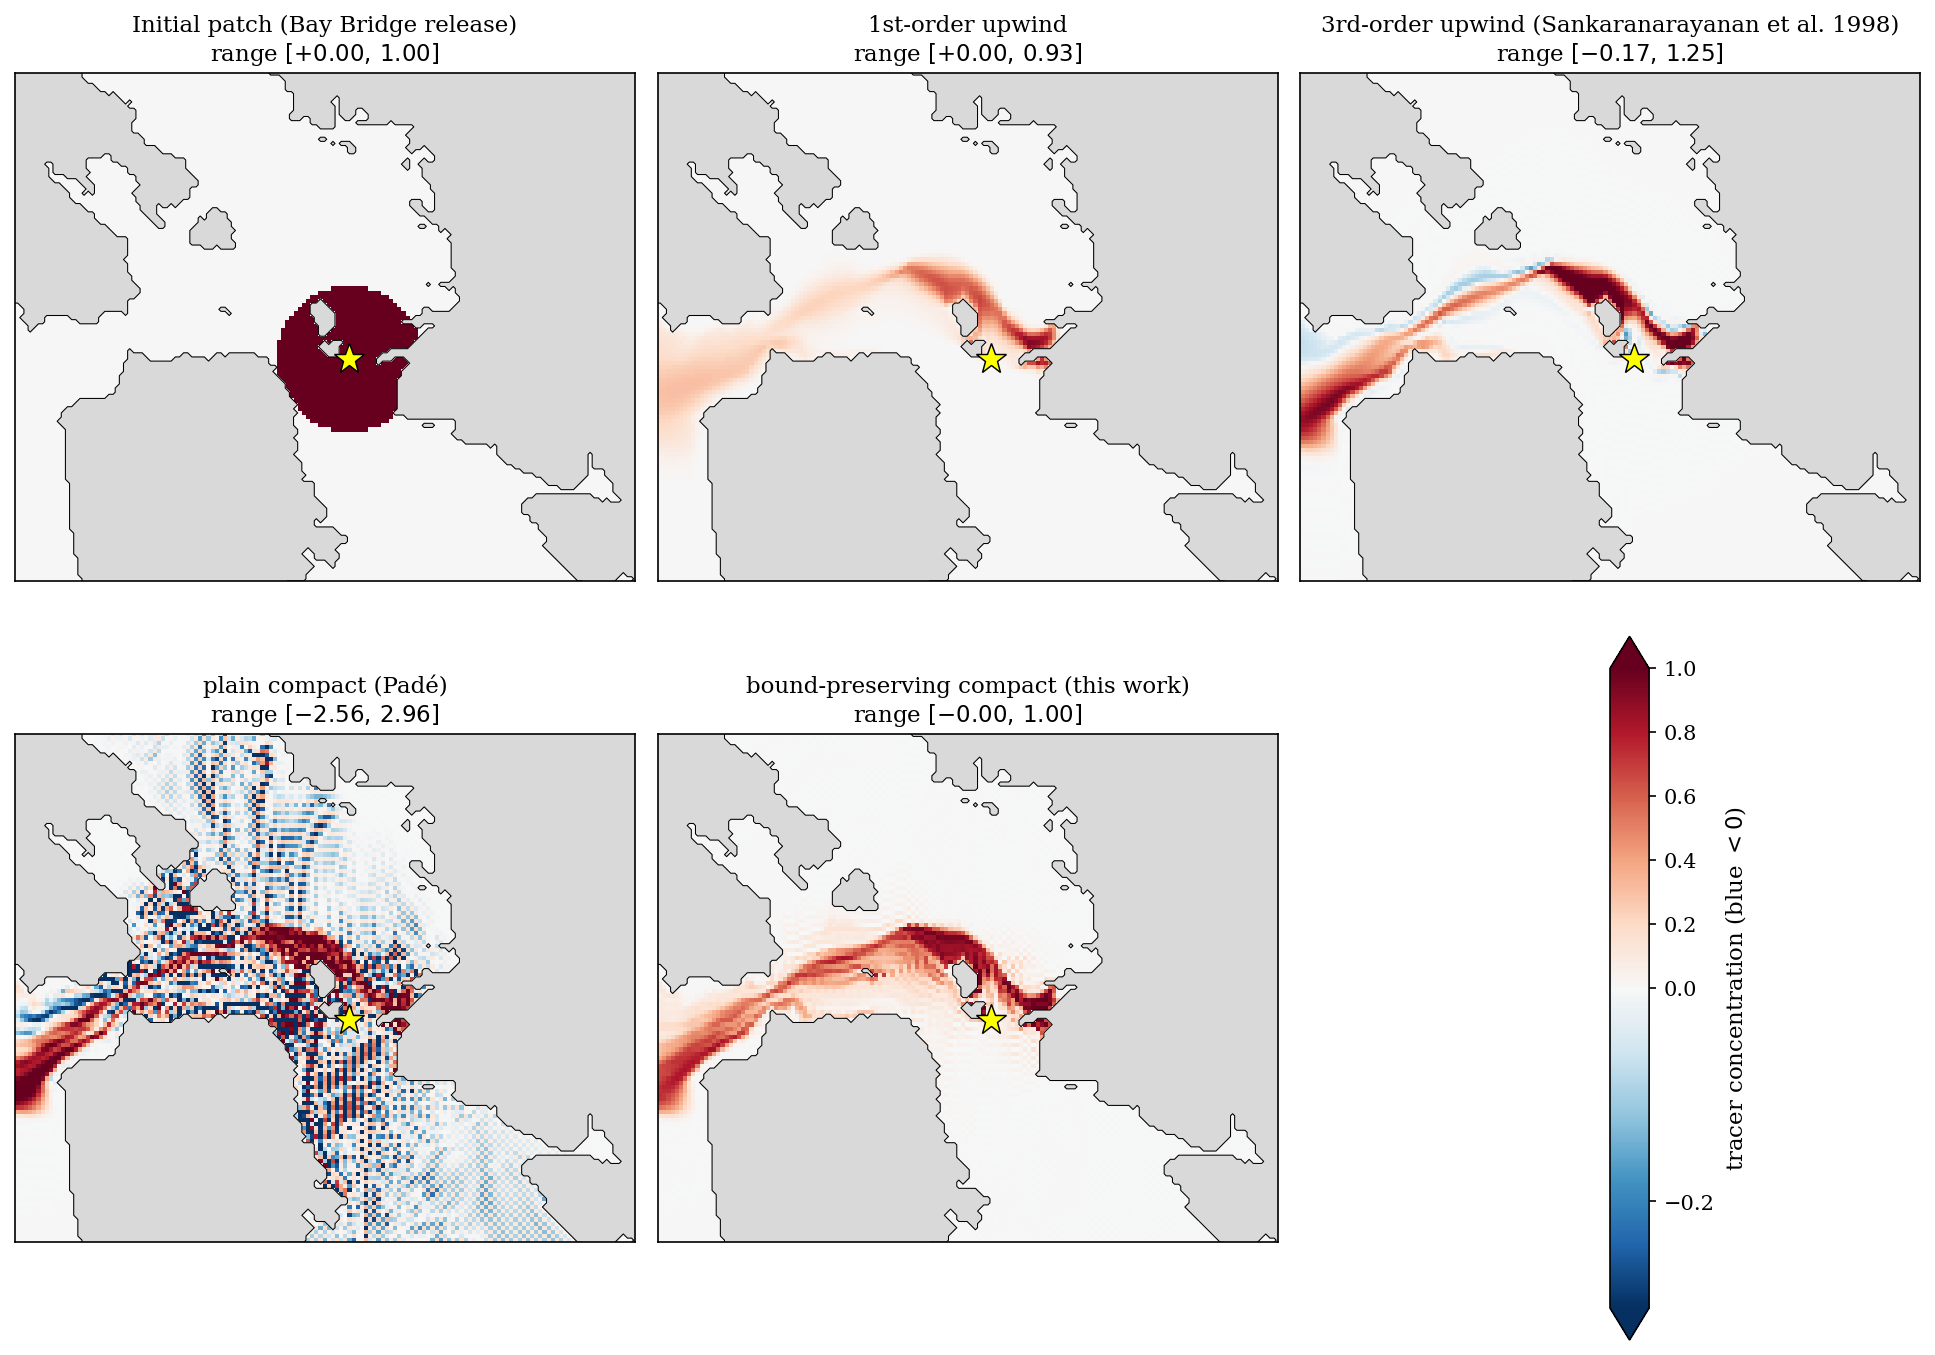
\includegraphics[width=\linewidth]{figures/fig_sfbay_transport.png}
\caption{Transport of a sharp tracer released at the \emph{Cosco Busan} spill site
in San Francisco Bay tidal currents (5~h, $200$~m grid; central-bay view). The
third-order upwind scheme of \citet{sankaranarayanan1998} and the plain compact
scheme produce negative concentrations (blue); first-order upwind smears the patch;
only the bound-preserving compact scheme remains in $[0,1]$.}
\label{fig:sfbay}
\end{figure}

\section{An expert-guided LLM workflow}
\label{sec:workflow}
Beyond the numerical results, a contribution of this paper is the workflow itself: a
reproducible, \emph{expert-in-the-loop} process for developing and validating a
civil/coastal-engineering computational model with a large language model (LLM).
\textbf{The author designed the study, made every scientific and modelling decision,
verified all results against observations and physical reasoning, edited and approved
the manuscript, and takes full responsibility for its content.} Claude Opus~4.8
\citep{anthropic2026claude} served as an implementation and drafting assistant under
the author's direction---performing coding, computation, plotting, and text drafting
from natural-language prompts---and is a tool, not an author. The cycle is summarized
in Fig.~\ref{fig:loop}.

\begin{figure}[t]\centering
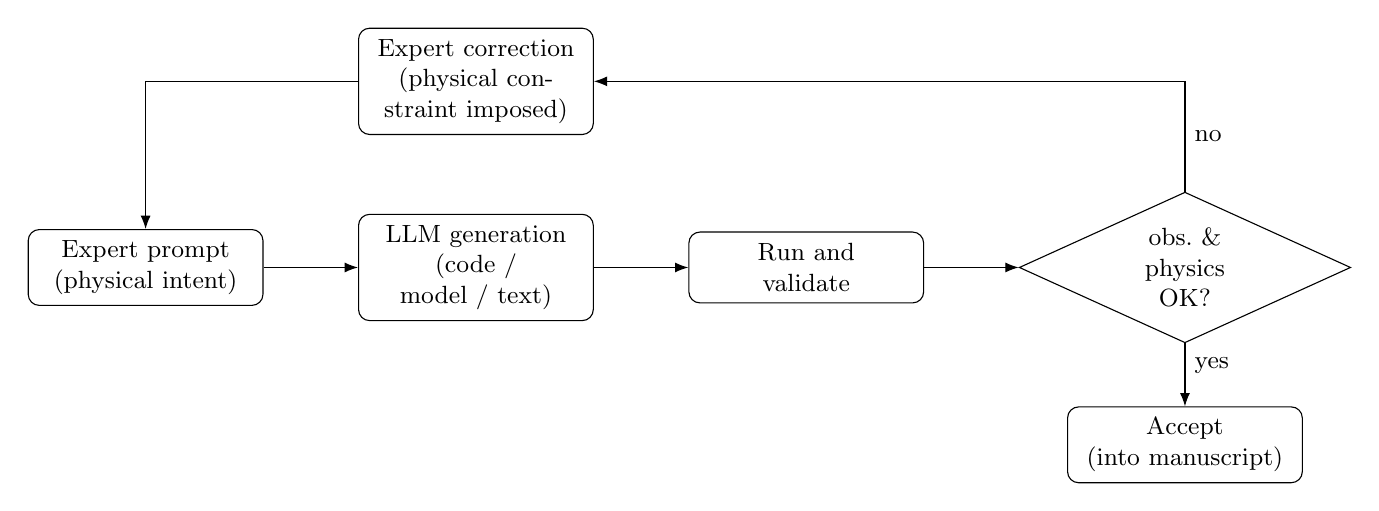
\begin{tikzpicture}[>=Latex, font=\small, node distance=7mm and 12mm,
  box/.style={draw, rounded corners, align=center, inner sep=4pt, minimum height=9mm, text width=27mm},
  dec/.style={draw, diamond, aspect=2.2, align=center, inner sep=1pt, text width=18mm}]
\node[box] (p) {Expert prompt\\(physical intent)};
\node[box, right=of p] (g) {LLM generation\\(code / model / text)};
\node[box, right=of g] (r) {Run and\\validate};
\node[dec, right=of r] (d) {obs.\ \&\\physics\\OK?};
\node[box, above=10mm of g] (c) {Expert correction\\(physical constraint imposed)};
\node[box, below=8mm of d] (a) {Accept\\(into manuscript)};
\draw[->] (p)--(g); \draw[->] (g)--(r); \draw[->] (r)--(d);
\draw[->] (d)--node[right,pos=0.35]{yes}(a);
\draw[->] (d) |- node[right,pos=0.25]{no} (c);
\draw[->] (c) -| (p);
\end{tikzpicture}
\caption{Expert-in-the-loop LLM workflow. The domain expert issues a physically
motivated prompt; the LLM generates code, model components, or text; the result is run
and validated against observations and physics; the expert either accepts it or
imposes a corrective physical constraint and re-prompts. Scientific decisions and
final responsibility remain with the expert.}
\label{fig:loop}
\end{figure}

\subsection{Expert correction of model errors}
Domain expertise, not the language model, governed the outcome
(Table~\ref{tab:workflow}). Several physically incorrect intermediate choices were
identified and corrected by the author on review: (i) a single-$M_2$ tide was replaced
by the six-constituent \emph{mixed} (semidiurnal $+$ diurnal) forcing required by this
estuary; (ii) an unphysically large minimum depth was replaced by a physical
$2$--$3$~m floor with depth-dependent (Manning) friction and a sponge layer to prevent
drying and instability; (iii) a coarse grid that over-concentrated the Golden Gate
current was replaced by a strait-resolving $200$~m grid calibrated to observed
harmonics; (iv) a domain trim that removed the tidal prism was reverted to the full
bay; and (v) an implied oil-spill hindcast was rescoped to an honest
tracer-transport demonstration. These corrections---spanning tidal forcing, numerical
stability, spatial resolution, volume conservation, and scientific scope---are failure
modes that only domain review catches, and are the substance of the human
contribution.

\subsection{Workflow evaluation and reproducibility}
The model was accepted only after passing independent validation against observations
(Table~\ref{tab:workflow}): Golden Gate $M_2$ elevation ($0.57$ vs.\ $0.58$~m) and
principal current ($0.96$ vs.\ $1.1$~m\,s$^{-1}$), the Oakland current ($0.53$ vs.\
$0.6$~m\,s$^{-1}$), the mixed-tide form factor ($\approx0.9$), a wet/dry stability
check (minimum water column $>0$ everywhere over the spring cycle), and the
deformational-benchmark boundedness separation. The complete pipeline---bathymetry
retrieval, grid generation, the calibrated mixed-tide solver, all figures, and the
symbolic order verification---is released as machine-runnable scripts plus a
structured \emph{skill} file that records, for each step, the driving prompt, the
imposed physical constraint, the script invoked, and the validation target, so the
study regenerates end to end. The implementation effort of this multi-component study
was compressed from the weeks such work typically requires to a few interactive
sessions; the value of the LLM lay in implementation throughput, while scientific
validity rested entirely on expert direction and verification.

\begin{table}[t]\centering
\caption{Evaluation of the expert-guided LLM workflow: expert-corrected errors,
independent validation checks the accepted model passed, and reproducibility artifacts.}
\label{tab:workflow}
\begin{tabular}{ll}
\toprule
Expert-corrected error & Correction imposed \\
\midrule
single-constituent ($M_2$) tide      & six-constituent \emph{mixed} forcing \\
unphysical minimum depth             & $2$--$3$~m floor $+$ Manning friction $+$ sponge \\
coarse grid (Gate over-concentration)& strait-resolving $200$~m grid, calibrated \\
domain trim (lost tidal prism)       & full-bay domain restored \\
implied oil-spill hindcast           & honest tracer-transport demonstration \\
\midrule
Independent validation check & Result \\
\midrule
$M_2$ elevation, Golden Gate & $0.57$ vs.\ obs.\ $0.58$~m \\
$M_2$ current, Golden Gate   & $0.96$ vs.\ obs.\ $1.1$~m\,s$^{-1}$ \\
$M_2$ current, Oakland       & $0.53$ vs.\ obs.\ $0.6$~m\,s$^{-1}$ \\
mixed-tide form factor       & $\approx0.9$ (mixed, predominantly semidiurnal) \\
wet/dry stability            & min.\ water column $>0$ (no drying) \\
deformational boundedness    & strictly bound-preserving in $[0,1]$ \\
\midrule
Reproducibility & end-to-end runnable scripts $+$ skill file $+$ calibration note \\
\bottomrule
\end{tabular}
\end{table}

\section{Conclusions}
\label{sec:conclusions}
We have applied a bound-preserving high-resolution compact finite-difference
scheme to the advective transport of a tracer in coastal and ocean flows, as a
follow-up to the conservative-pollutant transport model of
\citet{sankaranarayanan1998}. The scheme combines the spectral-like resolution of
the compact (Pad\'e) discretization with a stable no-flux boundary closure and an
a-posteriori discrete-maximum-principle limiter, the latter following established
bound-preserving practice \citep{zalesak1979,clain2011mood,lixiezhang2018}. On the
LeVeque deformational-flow benchmark and on tracer transport in San Francisco Bay
tidal currents, the scheme eliminates both classical pathologies of the advective
term: the unphysical negative concentrations of central and high-order upwind
schemes---including the third-order upwind scheme adopted in
\citet{sankaranarayanan1998}, which is shown here to produce negatives of order
$-0.2$ in realistic tidal currents---and the excessive numerical diffusion of
low-order upwind schemes, while conserving mass. The method is a practical
upgrade for the transport modules of operational coastal and ocean models, where
strict boundedness of salinity, temperature and pollutant concentrations is
required for stable coupling to biogeochemical and density computations.

\section*{Disclosure of AI use}
This study---the development and calibration of the hydrodynamic and tracer-transport
codes, the numerical experiments, the figures, and the drafting of this
manuscript---was carried out using the large language model Claude Opus~4.8
\citep{anthropic2026claude} as an implementation and drafting assistant, under the
direction and review of the author. The author designed the study, supplied the domain
expertise, took every scientific and modelling decision, verified all results, and
edited and approved the manuscript, and is the sole human author responsible for the
work; the language model is a tool and is not, and cannot be, an author. The workflow
and the expert corrections it required are described as a methodological contribution
in Section~\ref{sec:workflow}.

\section*{Data Availability Statement}
All code, data, scripts, the hydrodynamic calibration note, and the machine-executable
workflow (``skill'') file that support the findings of this study are openly available
in a public repository (archived at Zenodo, DOI to be assigned on acceptance; mirror
on GitHub), so that the entire study regenerates end to end. The input bathymetry
(NOAA NCEI Coastal Relief Model, Vol.~7) and the tidal harmonic constants (NOAA Tides
\& Currents, station~9414290) are publicly available from NOAA.

\section*{Acknowledgements}
Bathymetry is from the NOAA NCEI Coastal Relief Model; the Golden Gate tidal
harmonic constants are from NOAA Tides \& Currents (station~9414290).

%% (ascelike sets the bibliography style automatically)
\bibliography{references}
\end{document}
